% !TEX root = ../thesis.tex

%%%%%%%%%%%%%%%%%%%%%%%%%%%%%%%%%%%%%%%%%%%%%%%%%%%%%%%%%%%%%%%%%%%%%%%%%%%%%%%
% Chapter: Example Application
%%%%%%%%%%%%%%%%%%%%%%%%%%%%%%%%%%%%%%%%%%%%%%%%%%%%%%%%%%%%%%%%%%%%%%%%%%%%%%%
\chapter{Example Application: State Machine Monitoring}\label{Example Application}
In this chapter in order to show how our managed data implementation works in practice, and in particular in terms of aspect refactoring, we present a showcase.
The showcase consists of a very simple state machine application.
A similar example is presented in Enso paper as a showcase for its Object Grammar capabilities \cite{storm2012object}.

Consider the requirements of the state machine as the following: 
\begin{itemize}
	\item A state \texttt{Machine} consists of a number of named \texttt{State} declarations.

	\item Each \texttt{State} contains \texttt{Transitions} to other states, which are identified by a \texttt{name}, when a certain event happens.

	\item A \texttt{Transition} is identified by a certain \texttt{event}.
\end{itemize}

For reasons of simplicity, this example will be a very basic \textit{door state machine}, which includes three states \textbf{Open}, \textbf{Close} and \textbf{Locked}, accompanied by their transitions: \textbf{open\_door}, \textbf{close\_door}, \textbf{lock\_door} and \textbf{unlock\_door} respectively.
Figure \ref{fig:State_machine} illustrates the door state machine.

\begin{figure}[H]
	\centering
  	\fbox{\includegraphics[width=.50\textwidth]{figures/State_machine.png}}
  	\caption{Basic door state machine}
  	\label{fig:State_machine}
\end{figure}

To implement this we need to define the models, interpret the definition given a list of events and finally add any additional functionality (\textit{concern}) needed, for instance monitor the state of the door.

%%%%%%%%%%%%%%%%%%%%%%%%%%%%%%%%%%%%%%%%%%%%%%%%%%%%%%%%%%%%%%%%%%%%%%%%%%%%%%%
\section{Schemas definition}
As a first step, all the models of the state machine program need to be defined. 
An object diagram is illustrated in Figure \ref{fig:State_machine_object}.

\begin{figure}[H]
	\centering
  	\fbox{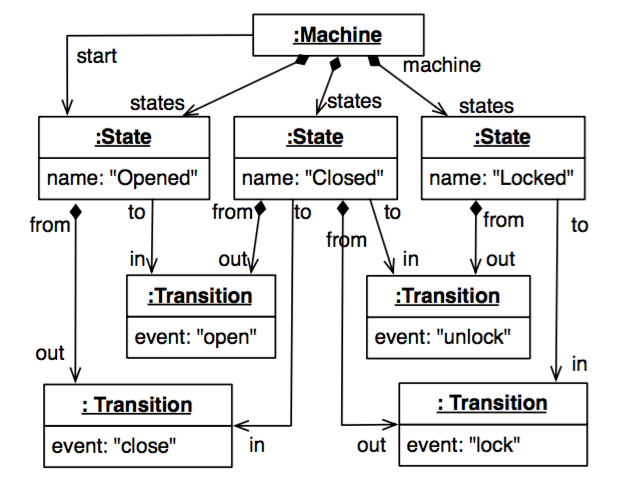
\includegraphics[width=.50\textwidth]{figures/State_machine_object_diagram.png}}
  	\caption{Basic door state machine object diagram}
  	\label{fig:State_machine_object}
\end{figure}

In our implementation we define schemas using Java interfaces with a set of meta-data described with Java annotations.
Therefore, as extracted from the requirements we need \texttt{Machine} (Listing \ref{lst:Machine_Schema}), \texttt{State} (Listing \ref{lst:State_Schema}) and \texttt{Transition} (Listing \ref{lst:Transition_Schema}) schemas.

%%%%%%%%%%%%%%%%%%%%%%%%%%%%%%%%%%%%%%%%%%%%%%%%%%%%%%%%%%%%%%%%%%%%%%%%%%%%%%%
\begin{sourcecode}[H]
	\begin{lstlisting}[language=Java,escapechar=|]
public interface Machine extends M {
	State start(State... startingState);

	State current(State... currentState);

	@Contain
	Set<State> states(State... states);
}
	\end{lstlisting}
	\caption{The Machine Schema}
	\label{lst:Machine_Schema}
\end{sourcecode}

As it can be seen in Listing \ref{lst:Machine_Schema}, the \texttt{Machine} schema definition requires a \texttt{start}ing state, the \texttt{current} state of the machine and a set of \texttt{states} that the machine can be into at each time.
Note that the \texttt{@Contain} annotation suggests that the \texttt{states} field is part of the spine tree and it is not a cross-reference.
This will be further explained in Chapter \ref{Implementation}.

%%%%%%%%%%%%%%%%%%%%%%%%%%%%%%%%%%%%%%%%%%%%%%%%%%%%%%%%%%%%%%%%%%%%%%%%%%%%%%%
\begin{sourcecode}[H]
	\begin{lstlisting}[language=Java,escapechar=|]
public interface State extends M {
	@Key
	String name(String... name);

	@Inverse(other = Machine.class, field = "states")
	Machine machine(Machine... machine);

	@Contain
	Set<Transition> out(Transition... transition);

	@Contain
	Set<Transition> in(Transition... transition);
}
	\end{lstlisting}
	\caption{The State Schema}
	\label{lst:State_Schema}
\end{sourcecode}

For the \texttt{State} definition, Listing \ref{lst:State_Schema}, we need a \texttt{name} field, which represents the name of the state. 
This \texttt{name} field has been annotated with the \texttt{@Key} annotation, which indicates uniqueness. 
The states field of Machine can be indexed by name.
Moreover, the schema includes a set of \texttt{in} and \texttt{out} \texttt{Transition}s.
Since those two fields are of type \texttt{Set}, one field of the \texttt{Transition} schema has to be marked as \textit{key}.
In this case, it is the \texttt{name} field (Line \ref{line:transition_key} Listing \ref{lst:Transition_Schema}).
Finally, the field \texttt{machine} represents the state machine that the state is part of. 
As it can be seen in the schema definition, Listing \ref{lst:State_Schema}, the \texttt{machine} field has been annotated with \texttt{@Inverse}, which indicates that this field is a reference to a field of another schema.
In this case, the \texttt{machine} field of \texttt{State} schema is a reference to \texttt{states} field of \texttt{Machine} schema.

%%%%%%%%%%%%%%%%%%%%%%%%%%%%%%%%%%%%%%%%%%%%%%%%%%%%%%%%%%%%%%%%%%%%%%%%%%%%%%%
\begin{sourcecode}[H]
	\begin{lstlisting}[language=Java,escapechar=|]
public interface Transition extends M {
	@Key 					|\label{line:transition_key}| 
	String event(String... event);

	@Inverse(other = State.class, field = "out")
	State from(State... from);

	@Inverse(other = State.class, field = "in")
	State to(State... to);
}
	\end{lstlisting}
	\caption{The Transition Schema}
	\label{lst:Transition_Schema}
\end{sourcecode}

Finally, in the \texttt{Transition} schema definition, Listing \ref{lst:Transition_Schema}, we need an \texttt{event} that corresponds to the event of the transition and is the \textbf{key} of that schema.
The \texttt{from} and \texttt{to} fields represent the state that the machine changes from and to respectively.
However, these are just references to the \texttt{State} schema (Listing \ref{lst:State_Schema}).

%%%%%%%%%%%%%%%%%%%%%%%%%%%%%%%%%%%%%%%%%%%%%%%%%%%%%%%%%%%%%%%%%%%%%%%%%%%%%%%
\section{Factory definition}
Now that we have our schemas, we need a way to build instances of managed objects that these schemas describe. 
In Java to create these three schemas as managed data we need to define a factory, which creates managed data instances (managed objects) for each of these schemas \ref{lst:StateMachineFactory}.
Note that the method definitions work as \texttt{Constructors} of managed objects.

\begin{sourcecode}[H]
	\begin{lstlisting}[language=Java,escapechar=|]
public interface StateMachineFactory {
	Machine Machine();  	// constructor for Machine managed objects
	State State(); 				// constructor for State managed objects
	Transition Transition(); // constructor for Transition managed objects
}
	\end{lstlisting}
	\caption{The StateMachine Factory}
	\label{lst:StateMachineFactory}
\end{sourcecode}

%%%%%%%%%%%%%%%%%%%%%%%%%%%%%%%%%%%%%%%%%%%%%%%%%%%%%%%%%%%%%%%%%%%%%%%%%%%%%%%
\section{Basic Data Manager}
As mentioned above, in order to interpret and manage the defined data we need data managers. 
Our implementation includes the definition of a \texttt{Basic data manager} that is responsible of interpreting a schema definition to instances of \textit{managed object}s.
Conclusively, in order to make a \textit{managed object}, the data manager needs its schema definition (the interfaces that define the schemas) and the schema factory (the interface that defines the constructors of the schemas).

%%%%%%%%%%%%%%%%%%%%%%%%%%%%%%%%%%%%%%%%%%%%%%%%%%%%%%%%%%%%%%%%%%%%%%%%%%%%%%%
\subsection{A simple without concerns program}
In the case of a simple program without any concerns, we have to use our managed data to define the state machine and then interpret it.
The definition of the door state machine is given in Listing \ref{lst:Door_state_machine} in Java.

In practice, the basic data manager needs to provide us with mechanisms that interpret the managed object that based on \texttt{stateMachineSchema}, shown in Line \ref{line:state_meaning_full_code}.
The basic data manager  also supports the field accessors of those data, namely, the setters and getters of their values.
An basic interpreter for the state machine is shown in Line \ref{line:state_machine_interpreter}.
As it can be seen, the schema factory is used to create managed objects.
The \textit{setup} of the fields is done automatically by the data manager who is responsible for the managed object interpretation.

\begin{sourcecode}
	\begin{lstlisting}[language=Java, escapechar=|]
public class StateMachineExample {
	public static void main(String[] args) {
		Schema schemaSchema = ...; |\label{line:state_schemaSchema}|
		Schema stateMachineSchema = ....; |\label{line:state_schemaMachineSchema}|
		BasicDataManager basicDataManager = 
				new BasicDataManager(StateMachineFactory.class, stateMachineSchema);  |\label{line:state_meaning_full_code}|
		StateMachineFactory stateMachineFactory = basicDataManager.make();

		Machine doorStateMachine = stateMachineFactory.Machine(); |\label{line:state_machine_creation_basic}|

		State openState = stateMachineFactory.State(OPEN_STATE);
		openState.machine(doorStateMachine);

		State closedState = stateMachineFactory.State(CLOSED_STATE);
		closedState.machine(doorStateMachine);

		State lockedState = stateMachineFactory.State(LOCKED_STATE);
		lockedState.machine(doorStateMachine);

		Transition closeTransition = stateMachineFactory.Transition(CLOSE_TRANSITION);
		closeTransition.from(openState); closeTransition.to(closedState);

		Transition openTransition = stateMachineFactory.Transition(OPEN_TRANSITION);
		openTransition.from(closedState); openTransition.to(openState);

		Transition lockTransition = stateMachineFactory.Transition(LOCK_TRANSITION);
		lockTransition.from(closedState); lockTransition.to(lockedState);

		Transition unlockTransition = stateMachineFactory.Transition(UNLOCK_TRANSITION);
		unlockTransition.from(lockedState); unlockTransition.to(closedState);

		doorStateMachine.start(closedState);

		interpretStateMachine(doorStateMachine, new LinkedList<>(Arrays.asList(
		        LOCK_TRANSITION,
		        UNLOCK_TRANSITION,
		        OPEN_TRANSITION)));
	}
}

private static void interpretStateMachine(
		Machine stateMachine, List<String> commands) 
{ |\label{line:state_machine_interpreter}|
    stateMachine.current(stateMachine.start());
    for (String event : commands) {
        for (Transition trans : stateMachine.current().out()) {
            if (trans.event().equals(event)) {
                stateMachine.current(trans.to());
                break;
            }
        }
    }
}   
	\end{lstlisting}
	\caption{Door state machine}
	\label{lst:Door_state_machine}
\end{sourcecode}

%%%%%%%%%%%%%%%%%%%%%%%%%%%%%%%%%%%%%%%%%%%%%%%%%%%%%%%%%%%%%%%%%%%%%%%%%%%%%%%
\section{Monitoring and notification concerns}
Consider a case in which we want to add concerns at the previous door state machine implementation.
A simple concern could be \textit{monitoring}, which would log every change in the current state of the state machine.
Another concern could be \textit{notification}, which would fire an action when a specific state is set.

Imagine that the system has to notify someone in case the door is opened.
If the door opens, then the \textbf{Open} state will be set as the current state of the machine.
In that case, a notification has to be sent by e-mail.
This looks similar to the \textit{monitoring} concern; however, in this case the notification is a specific action: send an e-mail in case the door opens.

\begin{figure}[H]
	\centering
  	\fbox{\includegraphics[width=.50\textwidth]{figures/State_machine_danger.png}}
  	\caption{Simple door state machine: notify closed door}
  	\label{fig:State_machine_danger}
\end{figure}

In order to implement those concerns we need a mechanism that continuously monitors the changes (transitions) of the machine's \texttt{current} state and reacts accordingly.
Usually, this would lead to scattered \textit{monitoring} and \textit{notification} code in the interpretation method or the models themselves (the machine model).
This is where data managers come to the rescue.
A data manager can implement concerns as modular aspects without crosscutting code to the components.
The programmer can define a manipulation mechanism of his/her data that includes an aspect of preference.
Therefore, by implementing our concerns with data managers we can keep the component and aspect code separate.

%%%%%%%%%%%%%%%%%%%%%%%%%%%%%%%%%%%%%%%%%%%%%%%%%%%%%%%%%%%%%%%%%%%%%%%%%%%%%%%
\subsection{Observable Data Manager}
Regarding the \textit{observation} of changes in the current state of our door state machine, we need a data manager that observes those changes in the managed object.
In particular, the \texttt{Machine}'s current \texttt{State} field.
This data manager creates concrete managed objects, namely \textit{observable managed objects}, where observes can be attached in order to be notified of changes.
It is important to mention that this new data manager has to inherit the basic one in order to include the basic functionality of schema interpretation and field access.
This leads to a \textbf{stack} of two data managers, each one adding a new aspect of data in a modular way.

%%%%%%%%%%%%%%%%%%%%%%%%%%%%%%%%%%%%%%%%%%%%%%%%%%%%%%%%%%%%%%%%%%%%%%%%%%%%%%%
\subsection{Monitor and notify concerns}
In the example the \textit{observers} are the concerns: \textit{monitoring} and \textit{notification}. 
Accordingly, the \texttt{current} state of the state machine is the \textit{subject} that informs the observers of its change.
The definition of the concerns is given in Listing \ref{lst:StateMachineMonitoring}.

\begin{sourcecode} [H]
	\begin{lstlisting}[language=Java, escapechar=|]
public class StateMachineMonitoring {
    public static void monitor(Object obj, String field, Object value) {
        if (field.equals("current")) {
            logger.log(" > Current state changed to " + ((State) value).name());
        }
    }

    public static void notify(Object obj, String field, Object value) {
        if (field.equals("current") && ((State) value).name().equals(OPEN_STATE)) {
            if (EmailSender.send("Danger!", "Someone just opened the door!")) {
            	logger.notify(" > Danger e-mail sent!.");
            }
        }
    }
}
	\end{lstlisting}
	\caption{Door state machine concerns definition}
	\label{lst:StateMachineMonitoring}
\end{sourcecode}

Since there is an observable data manager and the concerns are implemented in a separate and reusable module, completely unrelated to our logic code, we still need to integrate them in the original code.
The integration code is presented in Listing \ref{lst:StateMachineMonitoringConcerns}.
The only part that changes is Line \ref{line:state_machine_creation_basic} of the original code, where the data manager of the \texttt{Machine} managed object has changed to the new observable data manager.
Additionally, the concerns are attached to the machine object very easily, as can be seen in Lines \ref{line:state_machine_monitor} and \ref{line:state_machine_notify} of Listing \ref{lst:StateMachineMonitoringConcerns}.


\begin{sourcecode} [H]
	\begin{lstlisting}[language=Java, escapechar=|]
...
// State Machine monitoring
ObservableDataManager observableDataManager = 
			new ObservableDataManager(StateMachineFactory.class, stateMachineSchema);

StateMachineFactory observableStateMachineFactory = observableDataManager.make();

// Door State Machine definition, with observable data manager
Machine doorStateMachine = observableStateMachineFactory.Machine();

// Add monitoring and notification concerns
((Observable) doorStateMachine).observe(StateMachineMonitoring::monitor); |\label{line:state_machine_monitor}|
((Observable) doorStateMachine).observe(StateMachineMonitoring::notify);  |\label{line:state_machine_notify}|
...
	\end{lstlisting}
	\caption{Door state machine with concerns}
	\label{lst:StateMachineMonitoringConcerns}
\end{sourcecode}

By running the program with the commands \texttt{LOCK\_TRANSITION}, \texttt{UNLOCK\_TRANSITION} and \texttt{OPEN\_TRANSITION}, the output is presented in Listing \ref{lst:StateMachineMonitoringConcernsOutput}.
\lstdefinestyle{Bash} {
    backgroundcolor=\color{white},
    basicstyle=\scriptsize\color{black}\ttfamily
}

\begin{sourcecode} [H]
	\lstset{numbers=none}
	\begin{lstlisting}[style=Bash]
> Current state changed to Closed
> Current state changed to Locked
> Current state changed to Open
> Danger e-mail sent!
	\end{lstlisting}
	\caption{Door state machine with concerns: output}
	\label{lst:StateMachineMonitoringConcernsOutput}
\end{sourcecode}

The basic data manager allows to solely build managed objects, but the observable data manager also provides the functionality of attaching concerns in the managed objects after a specified event.
Concluding, the example presented a modular solution of \ac{ccc} without scattering and tangling code in the components.
